\begin{figure}%
	\centering%
	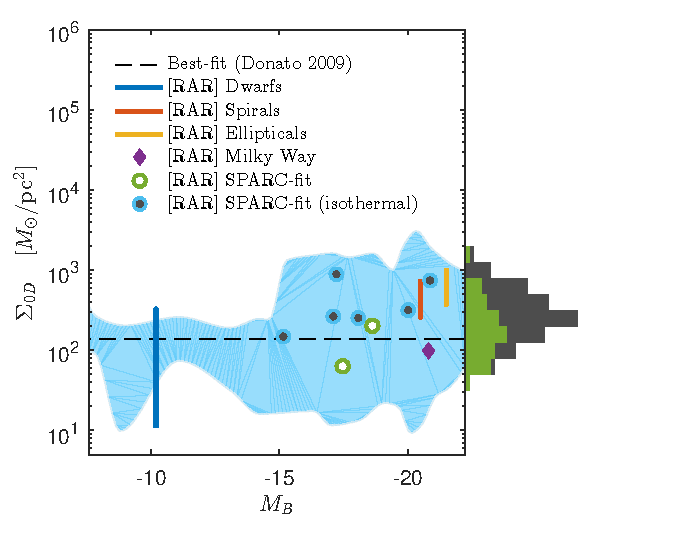
\includegraphics[width=\hsize]{\ROOTPATH/fig.pdf}%
	\caption{Rotation curves of the Milky Way galaxy. The observed velocities (black dots with error bars) are compared with the total velocity (thick solid line). The latter is composed of the baryonic component (dashed line), including a disk component (dot-dashed line), and the best-fit of the DM component, modeled with $50\mathrm{keV}$-RAR (thin solid line). For comparison, the NFW profile is added.}%
\label{fig:mw-rc}
\end{figure}